\chapter{Explaining Neural Networks}

% This section covers intro to explainablity of neural networks.
% We define aims and scope of explainability
% Why do we want to be able to explain models.
% some legal criterions
% some paper about patholigists not really believing the network. 
% We discuss utilized methods.

This chapter covers introduction to the growing field of explainable artificial intelligence. We start with short overview of the field itself, following by motivation for understanding decision of neural networks, alongside overview of legal obligations placed on decision support systems by European Union. We continue with overview of several explainability methods, suitable for our domain and task. This will serve as a foundation for the next chapter, where we evaluate selected methods against our benchmark.

In the contemporary literature, several terms are used when addressing the incomprehensibility of ML models. Arrieta et al. distinguish following idioms []:
% TODO - make actual definitions

\begin{enumerate}
    \item Understandability: Characteristic of a model to make a human understand its function without any need for explaining its internal structure or the algorithmic means by which the model processes data internally
    \item Comprehensibility: Ability of a learning algorithm to represent its learned knowledge in a human understandable fashion 
    \item Interpretability: Ability to explain or to provide the meaning in understandable terms to a human.
    \item Explainability: An accurate proxy of the decision maker and comprehensible to humans.
    \item Transparency: A model is considered to be transparent if by itself it is understandable.
\end{enumerate}

They further emphasize the distinction between interpretability and explainability -- interpretability, closely coupled with transparency are inherent and passive characteristics of a machine learning model. On the contrary, explainability is an initiated action taken to clarify model's internal details . Both can be seen as means to achieve understandability -- how a human can make sense of decisions made by the model [].

% https://pdf.sciencedirectassets.com/272144/1-s2.0-S1566253519X0007X/1-s2.0-S1566253519308103/main.pdf


\section{Need for understandability}

State of the art neural network models are often products of billions of parameters []. A term "black-box" models has been coined, to highlight their complex internal mechanics. In a crusade for ever-better performance and accuracy, models inherently grow in size and depth. Increasing size and complexity raises concerns of research community and general public, whether these networks can be trusted and used responsibly. [] []

% https://pdf.sciencedirectassets.com/272144/1-s2.0-S1566253519X0007X/1-s2.0-S1566253519308103/main.pdf
% https://ieeexplore.ieee.org/document/8400040

\subsection*{Spurious Correlations}
% systematic bias & reserch
Distrust does not stem only from lack of insight into model's internal reasoning. In certain cases, seemingly flawless performance of machine learning models may in fact be a result of a systematic bias in training and evaluation data. Commonly used example is an experiment by Ribeiro et al. where they purposely trained a logistic regression classifier to distinguish between wolves and husky dogs. The training dataset was arranged, such that wolf pictures have snow in their background and the husky counterpart does not. This led the classifier to make its decision based on the presence of snow in the picture, rather of the animal []. 

% husky - https://arxiv.org/pdf/1602.04938.pdf

Another, less artificial example is shown in Figure \ref{fig:horse-tag}. One can see, that a \emph{capable} model may produce a desired output, despite that the presence of features important for a human decision in input data had no influence on model's decision.

Instances such as these demonstrate that the understandability of a decision support system isn't just an issue for the end-user. It's also advantageous for the model's development cycle. Gaining insights into the factors influencing the model's decisions allows us to responsibly evaluate if its reasoning aligns with our expectations -- and take according measures if not.


\begin{figure}[!h]
    \begin{center}
    \begin{minipage}{1\textwidth}
      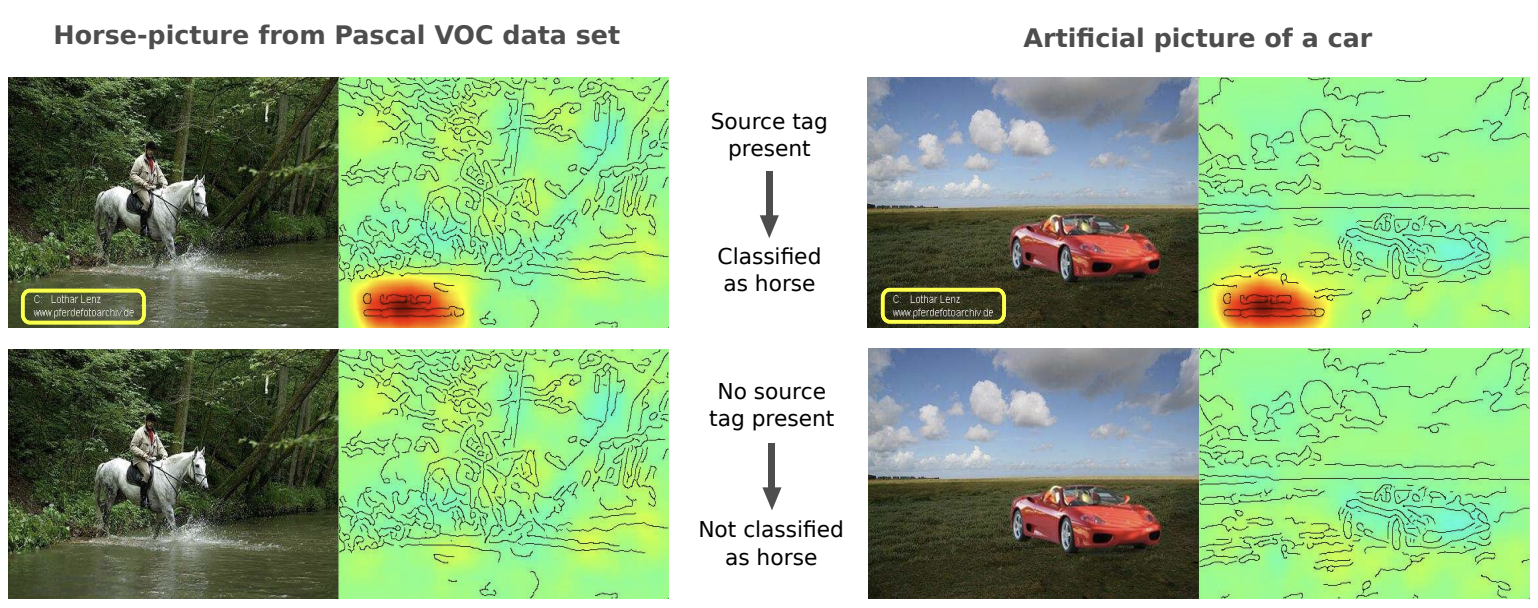
\includegraphics[width=\textwidth]{img/horse-tag.png}
    \end{minipage}
    \caption{Experiment conducted by Samek et al []. Model was trained on PASCAL-VOC dataset []. After the training, they found presence of so-called \emph{spurious correlation}. Pictures of horses are classified solely on whether the bottom-left corner of an input image contains a source tag. If the source tag manually added to an otherwise correctly classified image of a car -- the model changes its prediction, and the image is classified as a horse instead.}
    \label{fig:horse-tag}
    \end{center}

\end{figure}

% horse - https://arxiv.org/pdf/1902.10178.pdf

% medicine pov
\subsection*{Explainability in medical domain}

Such spurious correlations and the black-box tag lead clinicians to be sceptic about integrating AI in healthcare. Recent survey by GE HealthCare concludes, that out of 2000 clinicians participating in the survey, $58$ percent does not have overall trust in AI systems and $44$ percent of respondents believe, that the AI-based systems are biased []. Achieving trust of both clinicians and patients is crucial in order to achieve industry-wide utilization of machine learning-based systems.

% https://www.gehealthcare.com/about/newsroom/press-releases/ge-healthcare-reimagining-better-health-study-identifies-the-barriers-to-achieving-a-more-human-and-flexible-healthcare-experience



% legal
\subsection*{Legal obligations for AI explainability in the European Union}

Given certain applications, understanding the model is not only a moral obligation. In 2016, the European Union included what is often referred to as the "right to explanation" within the General Data Protection Regulation (GDPR). Specifically, Articles 13 and 14 give individuals the right to receive "meaningful information about the logic involved", when they are a part of automatic decision process making.  This pose a challenge for industry, implicating that adequate measures need to be taken in place in order to fully integrate decision support systems based on deep learning. More on what Articles 13 and 14 mean for AI is to be found in a paper by Goodman and Flaxman [].

% https://arxiv.org/pdf/1606.08813.pdf

Another piece of legislation from the European Union is anticipated to be implemented in May or June of 2024. \emph{AI Act} introduces a series of regulations for machine learning-based AI systems. The legislation is notably more detailed and exhaustive than Articles 13 and 14 of the GDPR, yielding mixed responses from domain experts. While the full implications are yet to be seen, it already imposes several restrictions on what needs to be met before deploying machine learning models. In particular, one section specifically targets high risk AI systems and states that a "Providers must build for human oversight, incorporating ‘human-machine interface tools’ to ensure systems ‘can be effectively overseen by natural persons’". Several other important aspects of model's life-cycle are revised as well, ranging from training dataset to technical documentation. Comprehensive overview of the article is beyond the scope of this thesis, and is summarized by Veale and Borgesius in [].

% https://www.degruyter.com/document/doi/10.9785/cri-2021-220402/html

\section{Explainable Artificial Intelligence}

Rapid development of deep learning models and scarcity of trust among users call for tools and methods, which allow us to understand and justify outputs of otherwise opaque systems. With the aim to shed light on internal processes of machine learning models, a sub-field of Explainable Artificial Intelligence (XAI) covers a range of techniques to make models more explainable, while preserving their performance and effectiveness. XAI techniques enable humans to build trust and manage machine learning based decision support systems -- a crucial part of assimilation of systems based on deep learning []. The exact borders of the field are not firmly set, and the notion of what does it mean to explain a model is an ongoing matter of discussion [].

\todo{find citations, forgot to write down}

Throughout this thesis, 'XAI' will refer specifically to the subfield dedicated to advancing explainability in AI, while 'explainable artificial intelligence' will denote the attribute of machine learning models that enables certain level of understandability. To describe explainable artificial intelligence, Arietta et al. [] suggest to use the following definition: \emph{Given an audience, an explainable Artificial Intelligence is one that produces details or reasons to make its functioning clear or easy to understand}.\newline
% taxonomy paper

\noindent
The field of XAI distinguishes between two means, how to make artificial intelligence understandable:

\begin{enumerate}
    \item Using transparent model: Models based on linear regression or decision trees are inherently interpretable -- therefore understandable by itself. By looking at their parameters, we are able to clearly derive, how they came to given conclusion.
    \item Using post-hoc explainability methods: When dealing with neural networks, we gain little insight into how they operate by simply inspecting their weights. Therefore we must implement auxiliary methods, which simplify and distill the reasoning of networks, so that according to the definition -- we get a clear and easy to understand explanation. Post-hoc explainability methods can be further divided into two subgroups -- global methods explaining model as a whole and local methods, focused on internal reasoning behind prediction for particular input sample.
\end{enumerate}

% Since neural networks can be seen as a complex non-linear attempt to approximate a function we cannot even fully define, it is easy to see that there is little to their transparent nature. If we want to better understand their decisions and reasoning, we need to carefully dive into post-hoc metods.
In the recent years, plethora of both global and local post-hoc explainability methods has been introduced in order to help grasp decision process of deep neural networks []. Post-hoc methods can be further divided into two groups. Model-specific methods are designed to explain only models with specific features and capabilities -- such as attention-based models or convolutional neural networks. On the contrary, model-agnostic methods can be used to explain arbitrary machine learning model.

\todo{lost citation}

% https://pdf.sciencedirectassets.com/272144/1-s2.0-S1566253519X0007X/1-s2.0-S1566253519308103/main.pdf
\section{Making CNN's explainable}




For convolutional neural networks, industry-wide standard is to visually highlight parts of a image, which are considered "important" to the model. The result of such visualization is commonly referred to as a \emph{saliency map}, class activation map (CAM) or attribution map. All terms mean 

SALIENCY MAP + class activation mapping (CAM)

\noindent
In following subsections we overview several explainability methods we will later benchmark in Chapter 4. We deliberately chose methods, which were not covered in previous work by RationAI's team. Popular methods such as LIME, Deconvolution or ...  were either computationaly too expensive, or produced sub-par results, which could not be used when deployed [].

\todo{cite matej and vojta}

\todo{ref chapter}
% attribution map vs saliency map

\subsection{Occlusion}

Occlusion is model-agnostic method and comes from family of so-called input perturbation based methods. Occlusion computes attribution map by systematically covering square parts in input image and observing the change in models prediction confidence on the perturbed image. Intuitively, we expect that when we cover (occlude) important part of the input image, the confidence of our classifier drops. In contrary, when we cover region which does not contain any important features, the output should not differ too much from output for the original pixel. Visual example can be seen in .... This approach gives us in dependence of the size of the square patch a rough heatmap of input feature saliency.

Experiment conducted by Gallo et al. [] shows, that in the domain of prostate cancer detection, the method produces semantically correct explanation maps. Sadly, occlusion comes with high computational complexity and resource utilization. For our use-case, explaining a single tile of $512px \times 512px$, the method needs 289 forward passes to compute the attribution map. 
% https://pdf.sciencedirectassets.com/277035/1-s2.0-S1871678423X00065/1-s2.0-S1871678423000511/main.pdf

In the production settings, size of the occlusion patch is 55 x 55 px and stride is set to 27 px. With those parameters in place, we need 289 forward passes through our our model to explain one patch. On a machine with 8 cores, 16GB of RAM and 48GB of GPU memory capacity, occlusion needs approx. 2 seconds and 40GB of GPU memory to generate single heatmap. Recall Section Y and processing WSI. In our test set, slide size varies from 400 to 4000 tiles per slide. Omitting auxiliary attribution map processing, this method takes  

\todo{Occlusion obrazok, ze je schopna zachytavat XPOi's a ze to su gleason patterns}

\subsection{CAM}

Zhout et al. show, that introducing GAP layer to a convolutional neural network has a welcome side-effect -- aside of regularization during trainig, it enhances networks localization capabilities, despite being trained on image level labes only. Their proposed method, called Class Activation Mapping (CAM) is used to visually highlight regions of input image used by the CNN to make its prediction for certain class $c$. This method is model-specific, since it works with networks having GAP (or GMP) as intermediate layer between the last convolutional layer and final fully-connected layer. 

On intuitive level, CAM is simply sum of weighted activations of last convolutional layer. To formalize, consider a network with convolutional layer with $F$ activation maps $A^1, A^2, ..., A^F$ followed by GAP layer and single fully connected layer, in which we fix neuron denoting class $c$. Recall Equation ..., and that GAP reduces value of each activation map $A^k$ to a single value $a^k$ -- average of the activations. The score for class $c$ is then calculated as:

\begin{equation}
    s^c = \sum_{k=1}^F a^k * w^k_c
\end{equation}

To define class activation map for class $c$, we use the same weights as in Equation .... Consider feature $A^k_{xy}$ in attribution map $A^k$, where $x$ and $y$ denote spatial coordinates of this feature. The mapping value is then calculated as follows:

\begin{equation}
    I
\end{equation}

We compute a kernel of mappings $K$ such that $K_{xy} = I$ for all pairs of $x, y$. Therefore $s^c$ is equal to the sum of  and directly indicates importance of the respective spatial locations.\newline

\noindent
Authors point out, that this method is particularly useful for networks with GAP layer. They believe that using GMP leads to the method pointing out to the single most discriminatory location, instead of all of them. While this has been largely confirmed by their experiment on ILSVRC dataset [], we believe that the method is worth considering for our use case. Models employed in the experiment are trained to distinguish between $1000$ classes, while their last convolutional layer had $1024$ filters. In our setting, the last convolutional layer has 512 units -- meaning there is hope that even though we only take the most discriminative location, averaging accross all units will lead to enough information when they only capture features for one class.

\todo{Toto je napisane uplne strasne, ale som uz unaveny.}



\subsection{GradCAM++}

GradCAM++ is popular gradient-based model-specific method used to spatially attribute convolutional layer features with respect to a given class. It improves upon its successful predecessor GradCAM []. We first overview th e GradCAM methods in order to see its limitations and how GradCAM++ specifically targets them.

% https://arxiv.org/pdf/1610.02391.pdf

GradCAM stands for Gradien-Weigthed class explanation maps. GradCAM is capable of explaining various CNN architectures, including VGG-16 based models. The idea is, that convolutional layer holds spatial information about their activation. Neurons in these layers look for certain patterns, and by their inspection, we should be able to point out, what are the model's areas of interest, given a input image and a class $c$.

Principle of GradCAM is fairly straightforward. Let $L$ be a fixed convolutional layer of our network with feature maps $A^1, A^2, ... A^n$, each with $Z$ features. We compute importance weight $w^c_k$ for feature map $A^k$ as gradient of $y^c$ with respect to that feature map. Individual gradients are global-average-pooled, yielding following equation []:
\todo{Why do we use raw score instead of softmaxed, if we do not perturb the image?}

\begin{equation}
    w^c_k = \frac{1}{Z} \sum_i \sum_j \frac{\delta y^c}{\delta A^k_{ij}}
\end{equation}

To obtain a coarse saliency map, we compute weighted combination of activations and their respective importance. $ReLU$ is applied over the heatmap to get only positive values advocating for important features with respect to class $c$ []:

\begin{equation}
    S^c_{GradCAM} = ReLU(\sum_k w^c_k A^k)
\end{equation}

If pooling layers are present in the network, the saliency map $S^c_{GradCAM}$ is smaller than input image. This is solved by simply upsampling the saliency map to image resolution.\newline

\todo{gradcam success and adoptations, maybe that it is generalization of CAM, which is shit, localization capabilities}

\noindent
Chattopadhyay and Sarkar [] built novel method on foundation of GradCAM while addressing some of its problems. They observed, that if multiple occurences of class of interest $c$ are present in the input image, localization capabilities of GradCAM gets worse. According to authors, this stems from using unweighted partial derivatives in Equation 3.1. If there are multiple occurences of class $c$, different feature maps may get activated, resulting in diluted and faded saliency map. They proposed generalized solution, equivalent in terms of computational performance.  

\todo{GradCAM vs GradCAM++ obrazok z original paperu, tie veci co som spominal vyssie}

GradCAM++ introduces weights to the computation of partial derivatives, slightly changing the Equation 3.1 into []:

\begin{equation}
    w^c_k = \sum_i \sum_j \alpha^{kc}_{ij} \times ReLU(\frac{\delta Y^c}{\delta A^k_{ij}})
\end{equation}

Thanks to additional coefficient $\alpha^{kc}_{ij}$ for all partial derivatives, all instances of class $c$ will be highlighted with equal importance. Inspiration for using $ReLU$ -- therefore taking only positive partial derivatives -- comes from Deconvolution and Guided Backpropagation, both being post-hoc methods already covered by Gallo et al. in []. Unlike GradCAM, GradCAM++ computes the partial derivative for activated score, as it needs it to be smooth function. This is denoted by $Y^c$ in Equation 3.3. For derivation of $\alpha$, visit third chapter of original GradCAM++ paper []. To obtain saliency map $S^c_{GradCAM++}$, we simply plug $w^c_k$ into Equation 3.2.

% https://arxiv.org/pdf/1710.11063.pdf

Being able to attribute all occurences of cancerous tissue would be a major advantage, since it is possible for a tile to contain multiple gleason patterns. Highlighting them all will undoubtledly lead to a greater trust of the examining clinician.
\todo{successful utilization of gradcam++, that it beats normal gradcam and so.}

\subsection{HiResCAM}

HiResCAM is another gradient based method building upon GradCAM's success. First step is the same as for GraCAM++ -- we need to compute partial derivatives of $y^c$ with respect to feature map $\mathcal{A}^k$ Instead of condensing "importance" of the feature map to a single value, we build kernel of partial derivatives $\mathcal{A}^k$ of the same dimension as the feature map $A^k$. Then we simply do pairwise multiplication of repective kernels and feature maps of last convolutional layer, yielding following equation []: 

\begin{equation}
    S^c_{HiResCAM} = \sum_k \mathcal{A}^k \odot A^k
\end{equation}
% https://arxiv.org/pdf/2011.08891.pdf

The rationale is that this better reflects how models "sees" the input image. This way, feature maps are scaled accordingly to the gradient, before summing them up to form the saliency map. Authors claim, that GAP-ing the partial derivatives in Equation 3.1 leads to blurring the effect of the gradient across feature maps. 

In addition to the method itself, authors present a proof of HiResCAM's capabilities. The proof shows, that for convolutional networks ending in one fully connected layer, HiResCAM guarantees to visually highlight all parts of input image which increase class score $y^c$, given we compute the saliency map for the last convolutional layer []. Unfortunately, the proof cannot be extended as is for our model introduced in Section .... While the model ends in one fully connected layer, it is separated from the last convolutional layer by intermediate global max pooling operation, which reduces each feature map to a single value. This breaks down the assumption that we can extract spatial information from the feature maps, since such information will be destroyed in the GMP operation. 

Authors show, that given a model has CAM architecture, HiResCAM saliency collapses to produce identical results as the CAM method from Section .... However, our model is using GMP instead of GAP, therefore the theoretical implications are unclear.

\subsection{ScoreCAM}

With aim to bridge gap between perturbation-based and gradient-based methods, Wang and Wang [] introduced ScoreCAM to fight with several problems introduced by GradCAM method. Unlike it is the case for previous CAM methods, ScoreCAM does not rely on gradient to compute the saliency. Instead, author relies on so-called increase in confidence $c_i$ for input vector $X$, which is defined by following equation:

\begin{equation}
    c_i = f(B \odot H_i) - f(B)
\end{equation}

Where $B$ is apriori known baseline vector, and Hadamard product with $H_i$ replaces $i$-th entry with $x_i$ from original input vector.

We use Equation ... to further define channel-wise increase in confidence:

\begin{equation}
    C(A^k) = f(X \odot scale(upsample(A^k)) - f(X_b)
\end{equation}

Where $upsample$ is a function, which resizes activation map $A^k$ to the size of input and $scale$ is scaling function to squish upsampled activation to range $[0, 1]$. $C(A^k)$ is then importnace score for unit $k$ given input $X$.

Then we calculate the final saliency map using channel-wise increase of confidence as our weight for convolutional layer activations, yielding []:

\begin{equation}
    L_{ScoreCAM}^c = ReLU(\sum_k C(A^k_l) \cdot A^k_l)
\end{equation}

As one of the initial goal of authors, we get rid of dependency of intermediat GAP (GMP) layer. According to the conducted experiments, ScoreCAM is able to locate multiple objects, something we believe might not be possible due to our utilization of GMP layer. In the original paper, authors also mention that saliency maps computed by ScoreCAM are more "focused" than the ones computed by GradCAM++. While having focused saliency maps is desired property, comparing results visually and drawing any conclusions is considered being an anectodal evidence and proper quantitative assessment needs to be done [].

% anecdotal evidence paper

\subsection{AblationCAM}

\todo{Gradient saturation}

Riding the wave of gradient free methods, AblationCAM utilizes ablation analysis to compute importance of feature maps. AblationCAM computes how inidividual feature maps contribute to the final score $s^c$, given class $c$ by iteratively removing them and observing drop in comfidence of the model. To replaces gradient, preventing gradient saturation or explosion. Influence of removal of feature map $A^k$ to final score is defined as:

\begin{equation}
    w^c_k = \frac{y^c - y^c_k}{y^c}
\end{equation}

The idea is, that if we remove filter important to the network when assessing presence of class $c$, the score should drop. To obtain the final saliency map, we compute the ablation weights for layer of interest, yielding the following equation:

\begin{equation}
    L^c_{AblationCAM} = ReLU(\sum_k w^c_k \cdot A_k)
\end{equation}

As it is the case for ScoreCAM, this method does not require gradient or GAP, and therefore it should be able to detect the occurrence of multiple instances of important input feature captured by feature map.

\subsection{Layer-Wise Relevance Propagation}

While Occlusion estimated feature importance by observing changes in output and CAM-based methods utilized spatial information in convolutional layer, Layer-Wise Relevance Propagation (LRP) takes different approach. Given a output score of the network, LRP utilizes several types of propagation rules to redistribute the score from output layer all the way down to the input pixels. Idea is, that we can look at how individual pixels contribute to the final score -- Each pixel value is weighted and sent to the upper layer across the whole network and in reverse fashion, we can compute the pixel importance.

To describe this procedure, assume $i$ and $j$ are two neurons in consecutive layers, such that there is and connection from $i$ to $j$. Process of relevance propagation is captured by following generic propagation rule:

\begin{equation}
    R_i = \sum_j \frac{z_{ij}}{\sum_i z_{ij} R_j}
\end{equation}

Where $R_i$ and $R_j$ are relevance scores and $z_{ij}$ models to which extent neuron $i$ contributed to neuron $j$'s activation []. The extent $z_{ij}$ is modeled by various rules, which are further described in []. The choice of rules is largely left to experimentation, however, Montavon et al. [] provide a blueprint for choosing layers when working with VGG-16. The main building block is LRP-$0$ rule:

\begin{equation}
    R_i = \sum_j \frac{a_i \cdot w_{ij}}{\sum_i a_i \cdot w_{ij}} R_j
\end{equation}

Where $a_j$ and $w_ij$ stand for activation and weight respectively, as defined in Section X.
\todo{ref section for weigh}

Gallo et al. used this rule exclusively on our model in [] and accordingly to observations of Montavon et al. in [], it lead to very noisy explanations. To tackle the noise, we add small positive term $\epsilon$ to the denominator -- $\epsilon$ will absorb weak and contradictory contributions, preserving only the salient scores. As a result, we typically get less noisy explanations. LRP-$\epsilon$ rule:

\begin{equation}
    R_i = \sum_j \frac{a_i \cdot w_{ij}}{\epsilon + \sum_i a_i \cdot w_{ij}} R_j
\end{equation}

To further enhance the explanations, LRP-$\gamma$ is used to favor positive contributions using coefficient applied only to the positive weights:

\begin{equation}
    R_i = \sum_j \frac{a_i \cdot (w_{ij} \cdot \gamma w_{ij}^+)}{\epsilon + \sum_i a_i \cdot (w_{ij} \cdot \gamma w_{ij}^+)} R_j
\end{equation}

For VGG-16, Montavon suggests to apply those rule in a very particular fashion, see Figure ...

\todo{Figure, explain rule selection on the bottom}